This section discusses a dynamic core composition scheme that is created by generating traces the ahead-of-time static compositions.
The section first describe how the traces are generated for the dynamic core composition schemes.
Before the analysis two types of static core composition are defined:

\begin{itemize}
	\item \textbf{Static Benchmark} (SB): A fixed fused-core which is optimal for a unique benchmark.
\vspace{-1.2em}
	\item \textbf{Static Suite} (SS): A fixed fused-core which represents the average best for the entire suite of benchmarks. This represents the baseline for the chapter.
\end{itemize}

The reason \textbf{Static Suite} is used as a baseline is due to the fact that it represents a configuration choice at design time.
It is the equivalent of hardware designers analysing the requirements of a processor based on the type of applications it will be executing.
This is better than using a single core as a baseline, as a single core will always represent the slowest execution time whilst also consuming the least amount of energy.
\textbf{Static Benchmark} on the other hand represents the ability to compose cores statically ahead of time; which is an extra step of flexibility compared to \textbf{Static Suite}.

The static core-composition scheme \textit{SS} is compared to the results obtained for the dynamic one for the SD-VBS benchmarks.
This is followed by a closer analysis of the dynamic core composition objective: optimising speed whilst reducing energy consumption.

\begin{figure}[t]
    \centering
	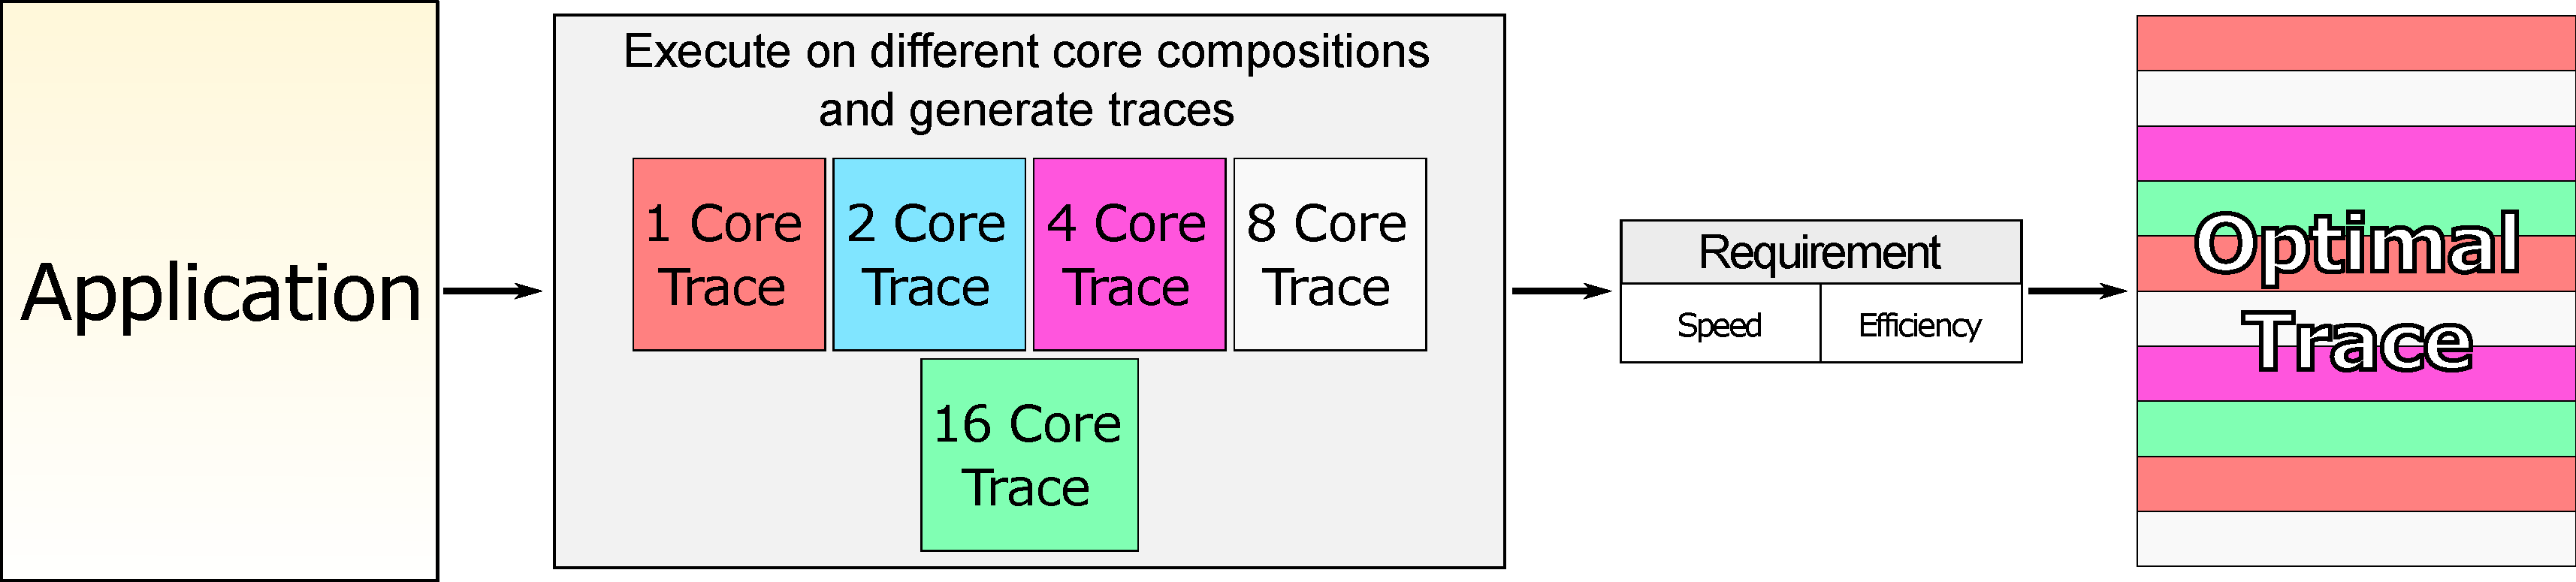
\includegraphics[width=1\textwidth]{cases-paper/graphics/exploration/trace-gathering.pdf}
    \caption{Overview of how traces are gathered to generate dynamic core composition traces.}
    \label{fig:tracegraph}
	\vspace{1em}
\end{figure}

\subsection{Creating Dynamic Core Composition Traces}

Dynamic core composition enables the ability to change the number of cores for each time tick (an interval of 640 committed blocks) during the execution of a program.
In order to explore the different performance and energy trade-offs that are possible to achieve with this technique, traces of execution for the application are collected.
Figure~\ref{fig:tracegraph} is a visual overview of how dynamic traces are collected.
First the application is executed on 1,2,4,8 and 16 composed cores and the performance is recorded for each time tick of 640 committed blocks.
Using these 5 traces, any dynamic execution can be constructed to generate dynamic traces.
For this chapter, the dynamic trace are generated based on maximising speed whilst minimising energy consumption.

To simplify the exploration process, time ticks that are attributed to the same phase are always given the same number of cores.
This is done to reduce the search space as on average there are 48,494 ticks which results in an average of $5^{48,494}$ different possible executions.
Since the maximum number of clusters found is 7 (for SVM), a maximum of $5^{7} = 78,125$ different dynamic execution traces can be built.
This is why creating dynamic core-composition out of traces is preferred to running all potential dynamic configurations via the simulator.
All applications run for a couple hundred million cycles, which often takes a couple of hours to execute.
As the amount of dynamic reconfigurations is high for some benchmarks, using traces to simulate dynamic reconfiguration is a very large time-save.

When the size of the core composition is switched, the performance of that composition from its respective trace file is used and an extra 100 cycle penalty is added for switching the size.
This 100 cycles is the overhead of reconfiguring the processor at runtime, the effect of the reconfiguration latency is discussed in further detail later on in this section.
The reconfiguration is a lightweight process as described in Chapter~\ref{chp:Background} section~\ref{sec:edge_arch} that involves informing the cores that they belong to a composition, which requires a write to a system register and potentially flushing pipelines if the cores are executing other threads.
As in this chapter, cores will never be executing other threads, flushing is not necessary, thus the l00 cycles to inform cores is an appropriate penalty and has been used in previous studies on DMPs~\cite{pricopi2012bahurupi}.
With all these different dynamic core composition traces, the optimal schemes for efficiently maximising speed can be found.

\begin{figure}[t]
    \centering
	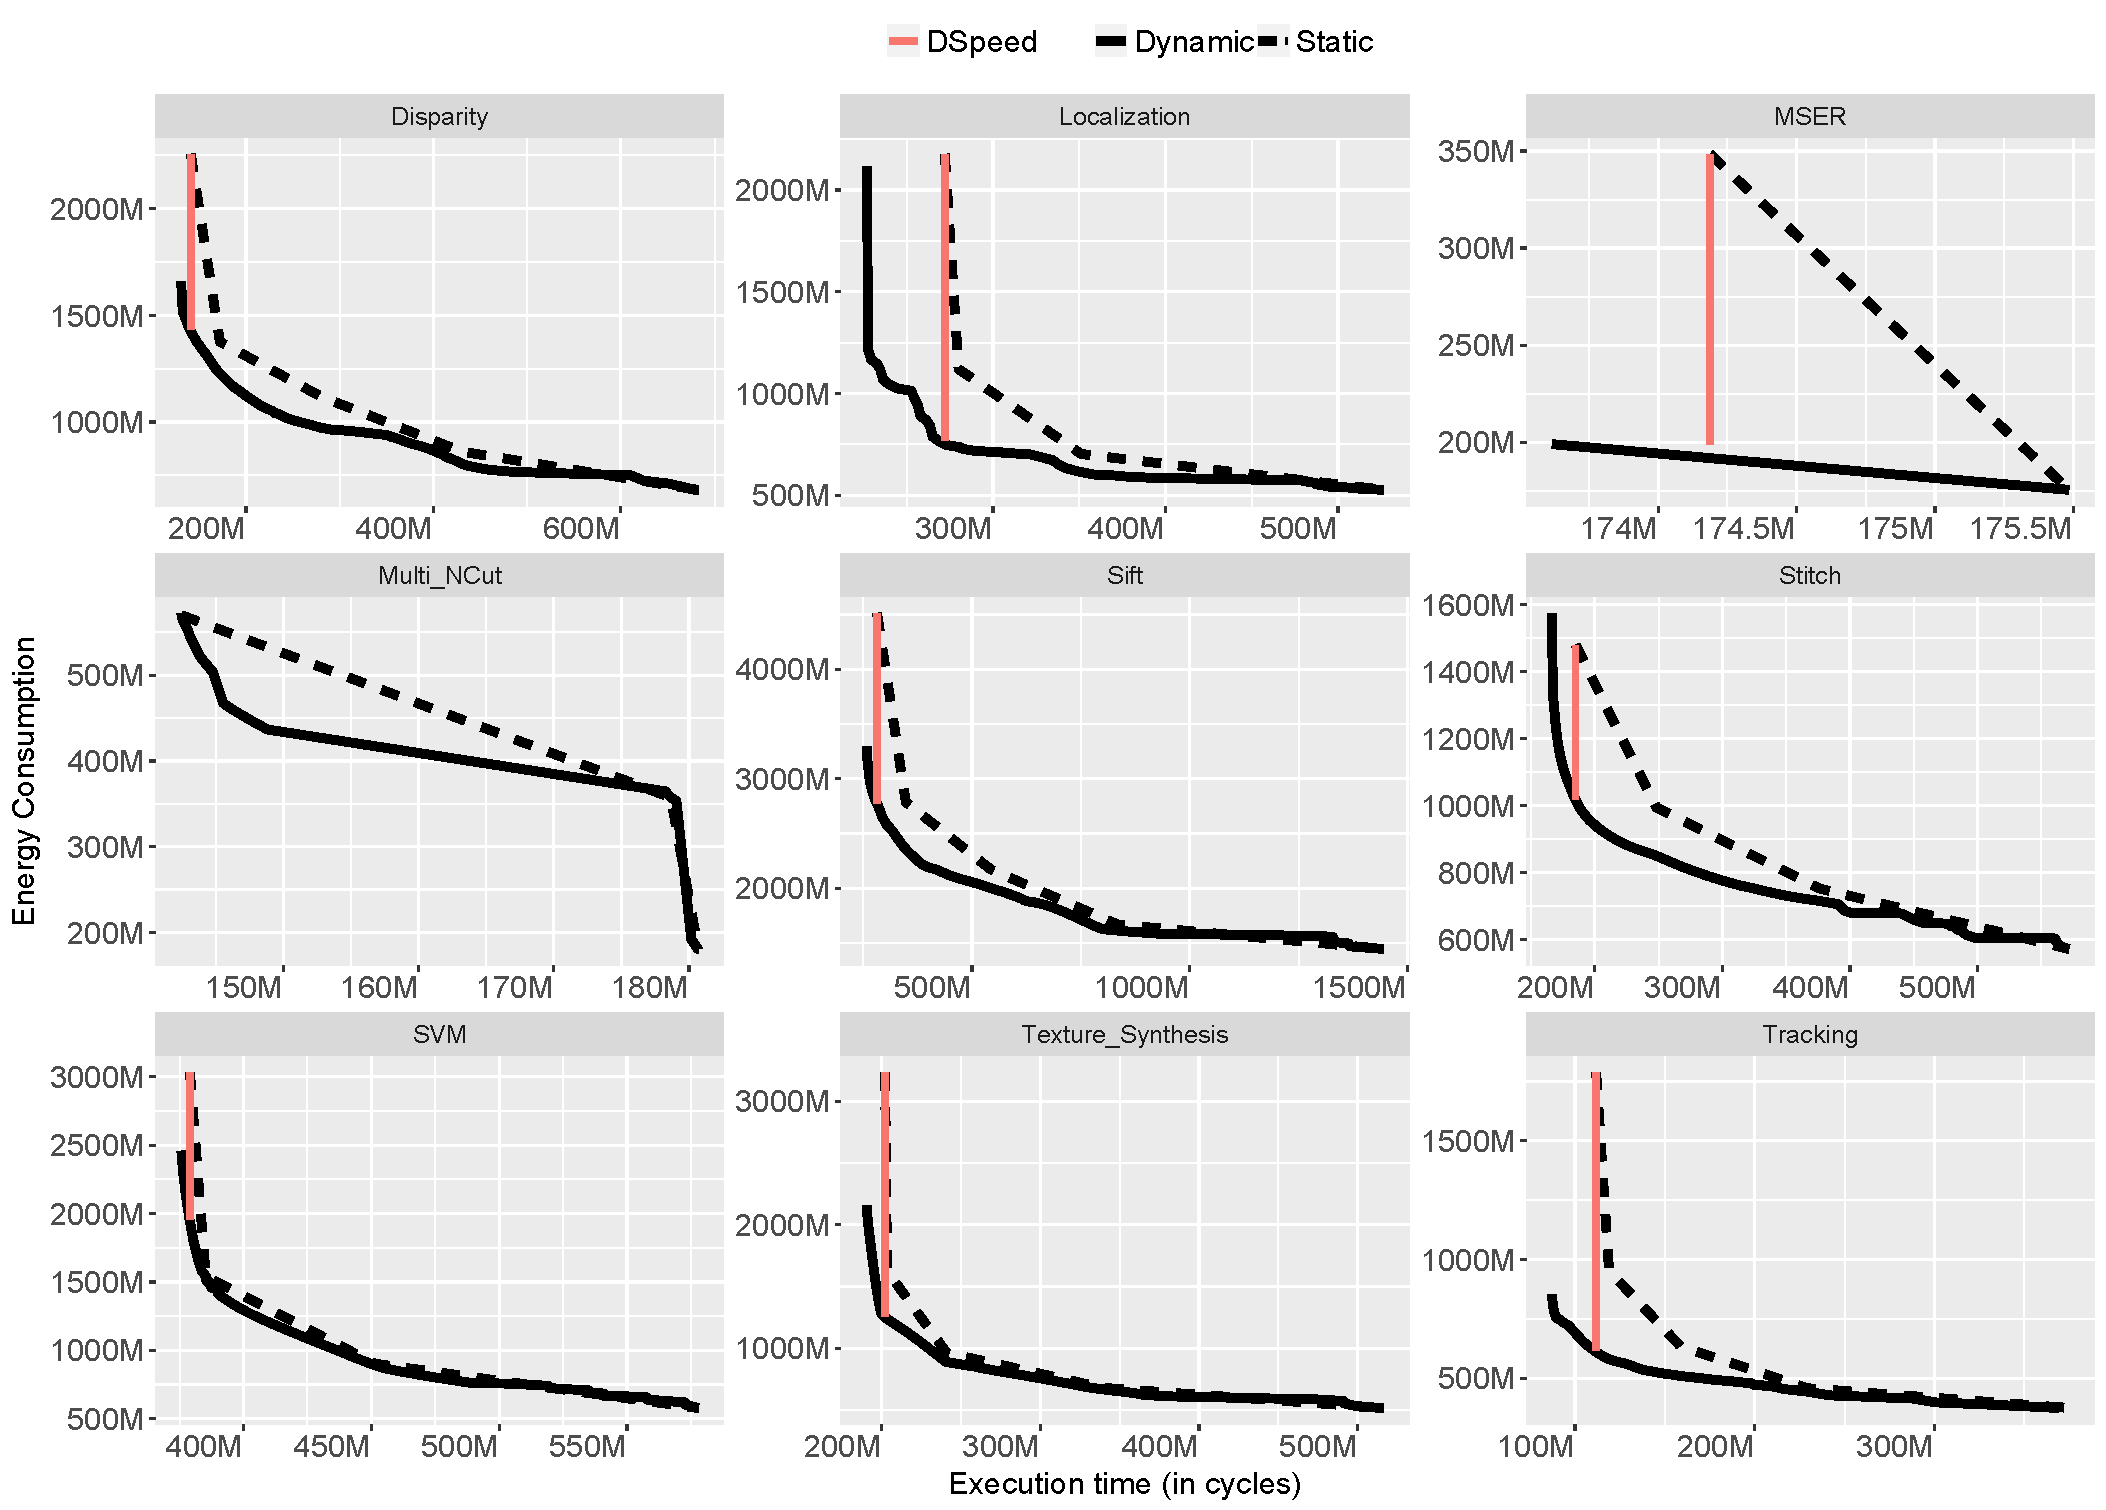
\includegraphics[width=1\textwidth]{cases-paper/graphics/pareto/pareto_best.pdf}
    \caption{Time (x-axis) vs. Energy (y-axis) trade-offs using Static and Dynamic Composition Schemes.}
    \label{fig:paretos}
	\vspace{1em}
\end{figure}

%\begin{figure}[t]
%     \centering	%
%	 \vspace{-1em}
%     \subfloat[][Disparity]{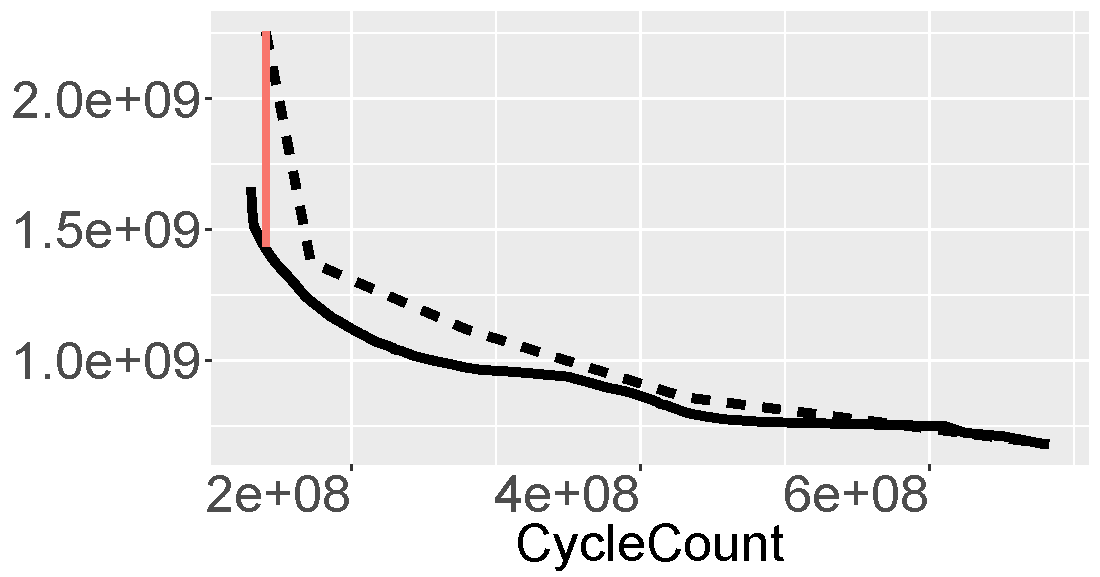
\includegraphics[width=0.33\textwidth]{cases-paper/graphics/Pareto/DispN3.pdf}\vspace*{-4mm}\label{subfig:disp}}
%     \subfloat[][Localization]{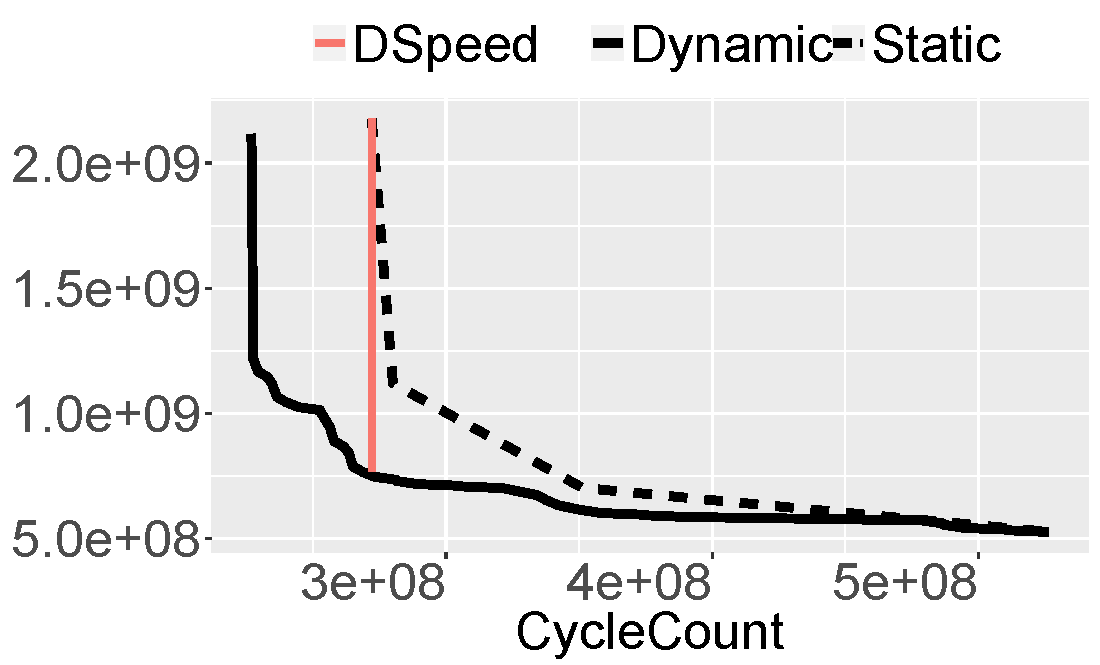
\includegraphics[width=0.33\textwidth]{cases-paper/graphics/Pareto/LocN3.pdf}\vspace*{-4mm}\label{subfig:loc}}
%     \subfloat[][MSER]{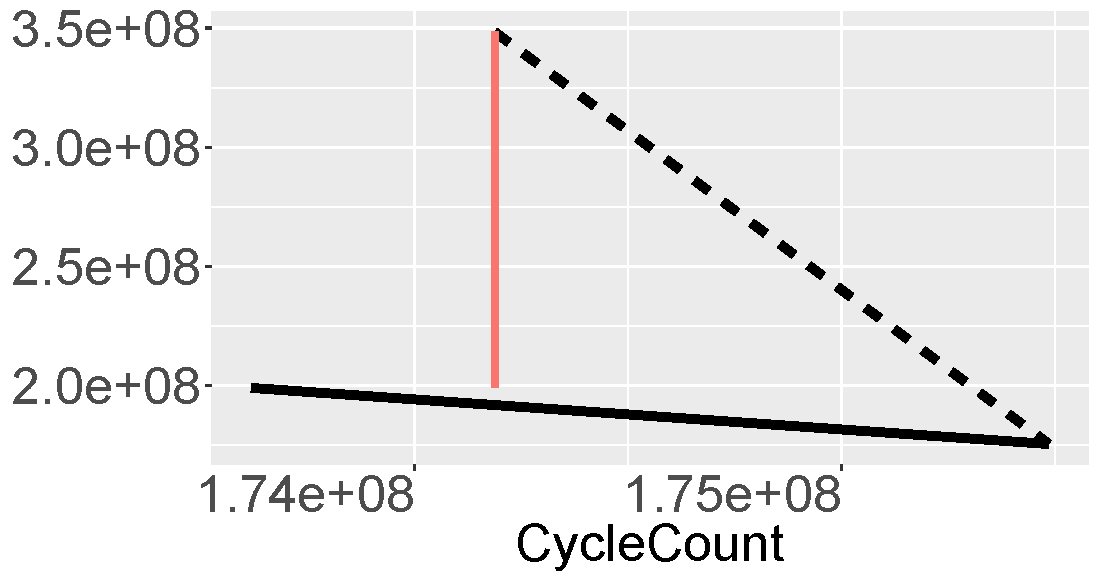
\includegraphics[width=0.33\textwidth]{cases-paper/graphics/Pareto/MSERN3.pdf}\label{subfig:mser}}\
%	 	 	 \vspace{-0.5em}
%
%     \subfloat[][Multi\_Ncut]{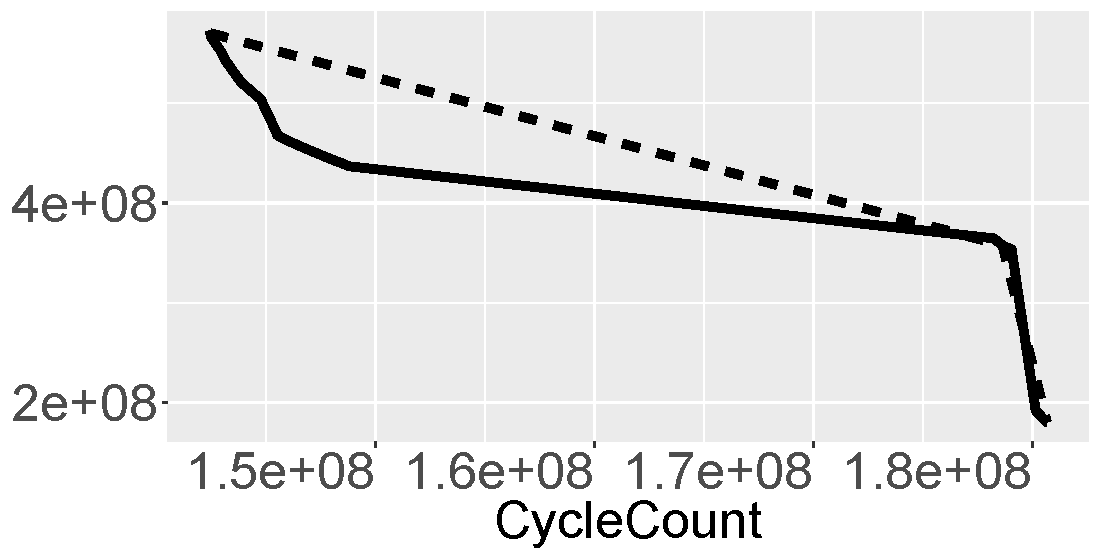
\includegraphics[width=0.33\textwidth]{cases-paper/graphics/Pareto/MultiN3.pdf}\label{subfig:mult}}
%     \subfloat[][Sift]{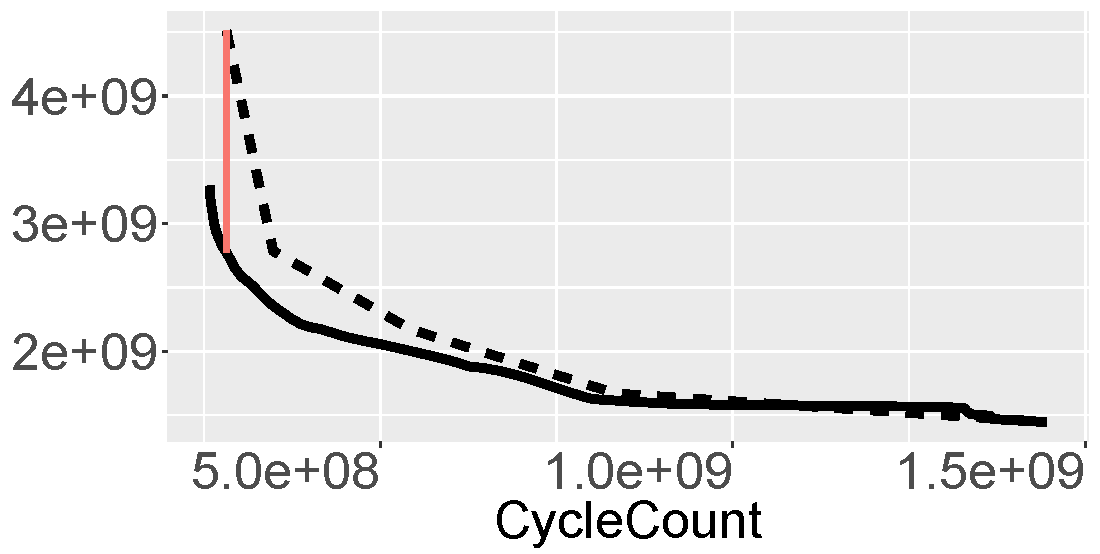
\includegraphics[width=0.33\textwidth]{cases-paper/graphics/Pareto/SiftN3.pdf}\label{subfig:sift}}
%     \subfloat[][Stitch]{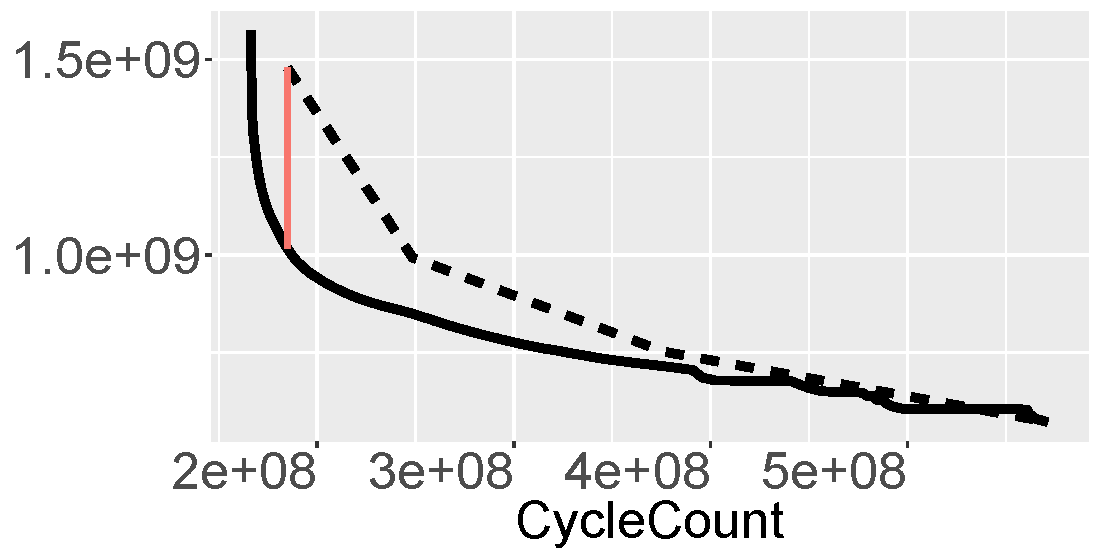
\includegraphics[width=0.33\textwidth]{cases-paper/graphics/Pareto/StitchN3.pdf}\label{subfig:stitch}}\
%	 	 	 \vspace{-0.5em}
%
%     \subfloat[][SVM]{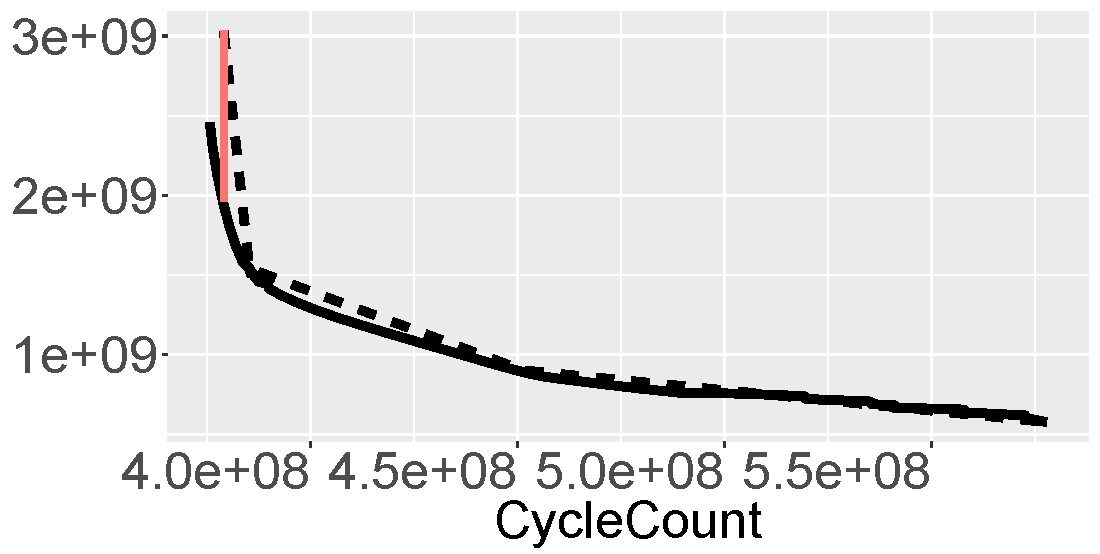
\includegraphics[width=0.33\textwidth]{cases-paper/graphics/Pareto/SVMN3.pdf}\label{subfig:svm}}
%     \subfloat[][Texture\_Synthesis]{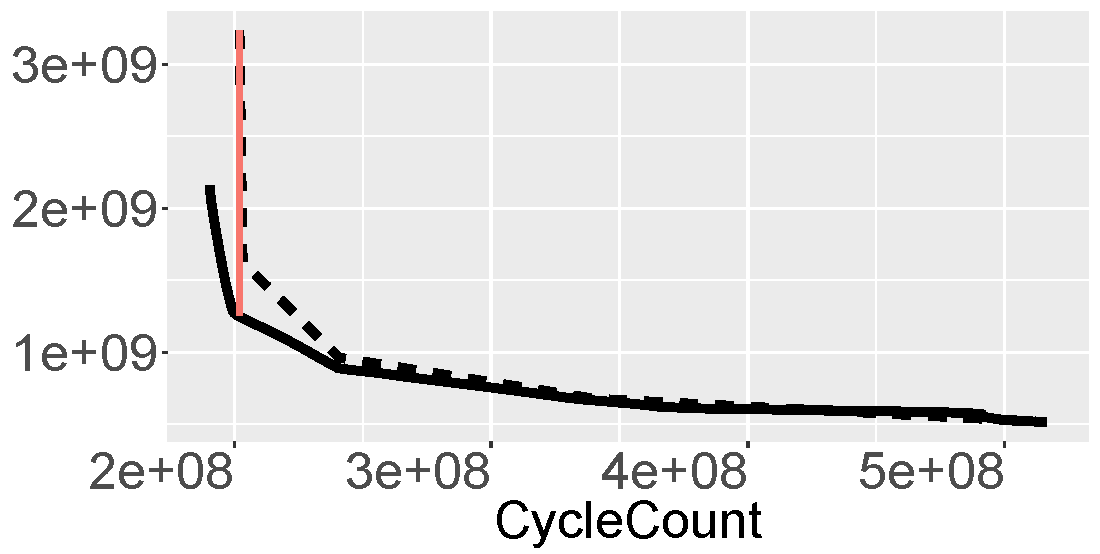
\includegraphics[width=0.33\textwidth]{cases-paper/graphics/Pareto/TextN3.pdf}\label{subfig:text}}
%     \subfloat[][Tracking]{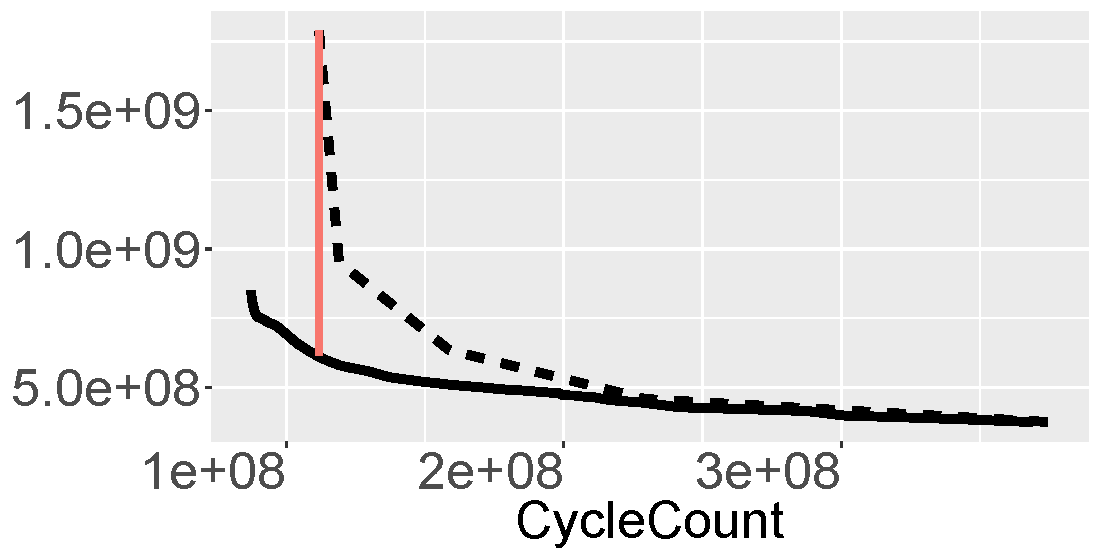
\includegraphics[width=0.33\textwidth]{cases-paper/graphics/Pareto/TrackingN3.pdf}\label{subfig:track}}
%     \caption{Time (x-axis) vs. Energy (y-axis) tradeoffs using Static and Dynamic Composition Schemes.}
%     \label{fig:paretos}
%	 	 	 	 \vspace{1em}
%\end{figure}

\subsection{Dynamic Core composition}
Figure~\ref{fig:paretos} shows the trade off between time (cycles) and energy using either a static ahead of time or dynamic (re)-configuration.
The dotted line represents the static core composition scheme for the benchmark whilst the solid line represents the Pareto Front of all the dynamic core composition traces.
The vertical line represents the amount of energy that can be saved from using a dynamic core composition scheme that matches the same speed as the best static scheme.
The Pareto Front is constructed by assigning different core composition sizes to a phase and recording the execution time in cycles and energy consumption.
For a given cycle count, the reconfiguration scheme that leads to the smallest energy consumption is chosen to be a point in the Pareto Front.

Figure~\ref{fig:paretos} demonstrates how static core-composition fails to maintain good energy efficiency as speed is improved.
For example, \bm{Disparity} is fastest on 16 fused cores, but has an 1.63x increase in energy consumption for a 1.22x improvement in speed.
This is due to the fact that larger core compositions do not result in linear speedups, and thus consume more energy than a smaller core composition.
When using the dynamic scheme, it is clear that energy consumption increases at a slower rate when increasing speed.
In this case the number of cores is adapted to the current phase, using just enough cores to maintain high performance without wasting energy.

Figure~\ref{fig:paretos} also shows how very few applications get faster execution times with dynamic core composition.
The main program that does perform better execution wise with dynamic core composition is \bm{Localization}.
In the case of \bm{Localization}, the fastest execution time using static core-composition comes from a logical core of size 8.
However, there are certain phases that perform better with 16 cores, and thus, dynamic core composition in this situation can lead to faster execution times.
Overall, for these benchmarks, most have their fastest execution times with a static core-composition.
Dynamic reconfiguration is therefore mainly used to limit the energy consumption.

\subsection{Optimising for Speed} \label{sec:dyn:speed}

In this section the dynamic scheme is defined to be one that matches the same speed performance as the fastest static core composition for the benchmark: \textbf{DSpeed}.
This is equivalent to the vertical line found in Figure~\ref{fig:paretos}.
This scheme is used to demonstrate how dynamic reconfiguration can achieve the same speed as the static configuration whilst reducing energy consumption.

Figure~\ref{fig:speedres} shows the speedup of \textbf{DSpeed} and Static Best (SB) and the respective energy consumption.
The results are normalized against the performance of Static Suite (SS), which is 8 cores fused.
The SS core count is obtained by averaging the number of cores that leads to the fastest execution time for each benchmark.
The execution times for \textbf{DSpeed} and SB are the same as the dynamic scheme is designed to match the static best's execution time.
As can be seen some benchmark perform better when using benchmark specific core compositions rather than SS.
Both \bm{Disparity} and \bm{Sift} obtain a 1.25x speedup when using the SB scheme whilst \bm{Tracking} benefits from a 1.10x speedup.
This reconfirms the concept that even static core-composition is a feature that leads to performance improvements over design time configurations.

\begin{figure}[t]
    \centering
	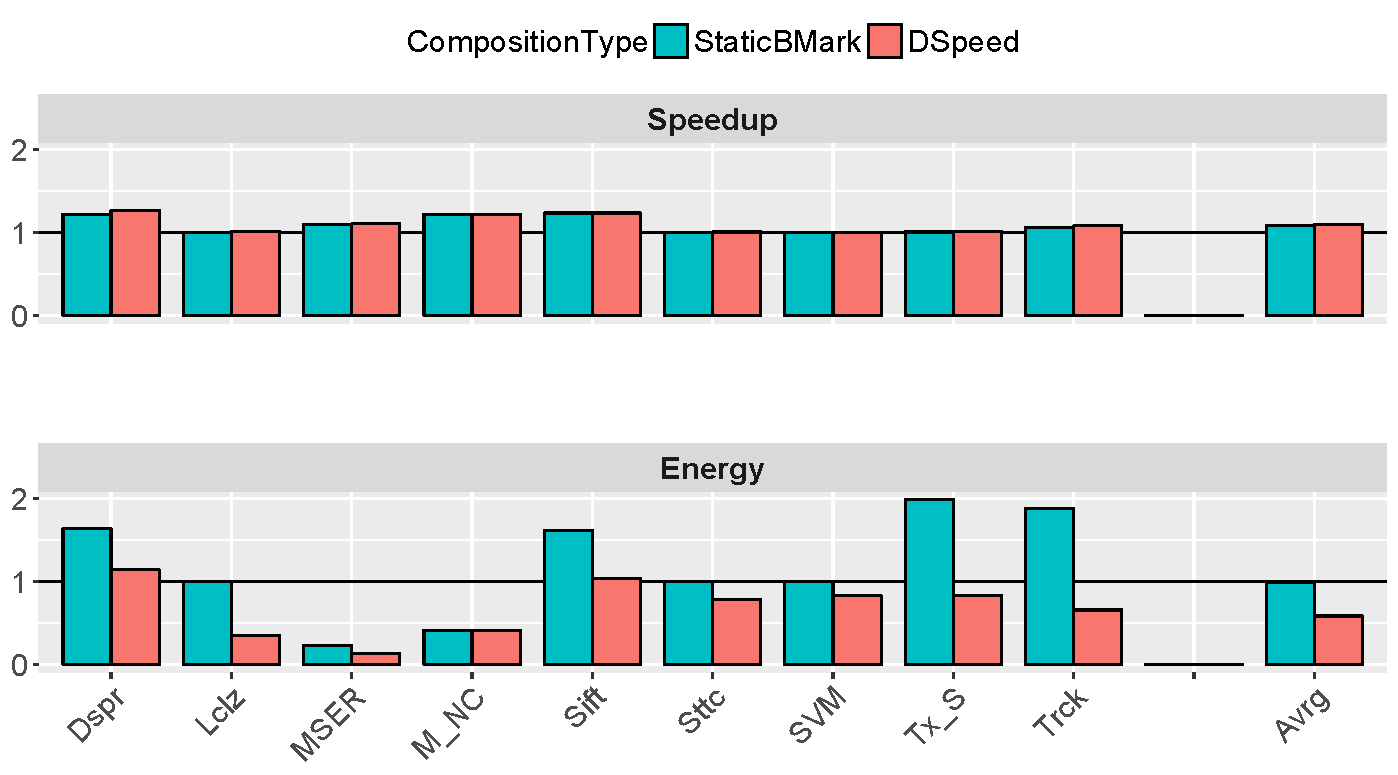
\includegraphics[width=1\textwidth]{cases-paper/graphics/results/speed_bars3.pdf}
    \caption{Maximising speed for all the SD-VBS benchmarks. For Speedup, higher means better, for Energy, lower is better.}
    \label{fig:speedres}
	\vspace{1em}
\end{figure}

When looking at the Energy graph of Figure~\ref{fig:speedres}, it is clear where the SS scheme fails.
Benchmarks \bm{MSER} and \bm{Multi\_NCut} feature very little improvements when using core composition, if any, therefore the SS will perform very poorly when it comes to energy consumption for the benchmarks.
In the case of those benchmarks, the energy consumption is over 2x less on SB than it is on SS.
In this situation, SS is analogous to designing a large physical core meant to extract a lot of IPC for single-threaded performance and executing low IPC benchmarks on it.
This core will end up consuming too much energy and lead to low performance increases.
SB already shows the advantages of designing smaller, simpler physical cores which can be composed ahead of time.
For applications such as \bm{MSER} or \bm{Multi\_NCut}, a single low energy core suffices whereas \bm{Disparity} and \bm{Tracking} benefit from large compositions for better speedup.

However, SB is still not an optimal solution. 
For the benchmarks \bm{Disparity}, \bm{Sift}, \bm{Texture\_Synthesis} the energy consumption is much higher.
This is due to the fact that these benchmarks perform best on a 16-core system, however as seen in Figure~\ref{fig:stddev}, the variation in performance always increases when fusing this many cores.
In this situation, whilst 16 cores does result in the fastest execution times, the energy consumption is higher than SS.
This shows the limitations of static configurations overall, whether it be at design time or ahead of time: the lack of flexibility means that compromises have to be made.
In the case of aiming for the fastest execution times energy consumption may increase.

%More here
The dynamic reconfiguration \textbf{DSpeed} scheme always performs better than the SB scheme in terms of energy consumption and can even match the SS scheme on energy consumption whilst improving speed such as in the \bm{Sift} benchmark.
For the \bm{Localization} benchmark, the \textbf{DSpeed} matches the performance of both the SB and SS whilst reducing energy consumption by 65\%.
By using \textbf{DSpeed}, the energy consumption can be reduced by 42\% compared to both SB and SS without impacting performance.
This illustrates the greatest advantage of using a DMP since the number of composed core can be adapted continuously depending on the amount of ILP available.

\subsection{Reconfiguration Latency} \label{sec:reconfoverhead}

\begin{figure}[t]
	\begin{minipage}{.5\textwidth}
	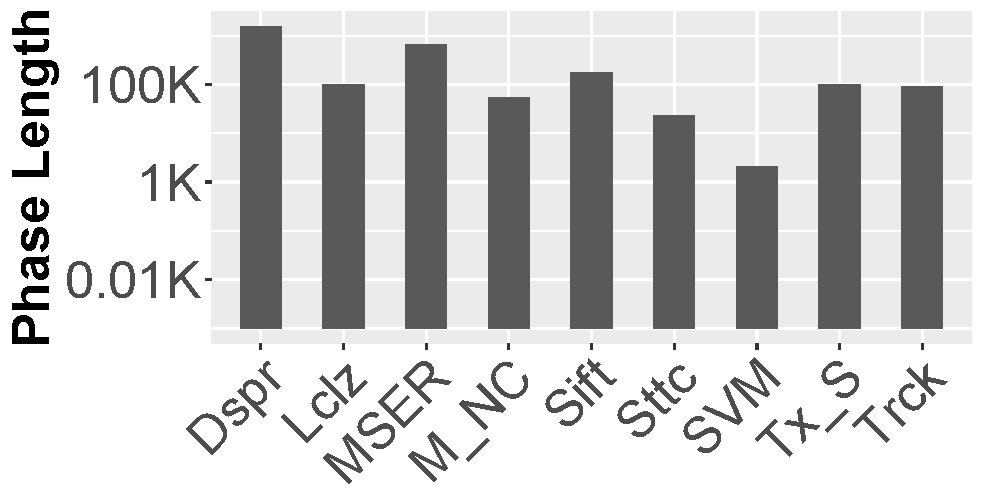
\includegraphics[width=.9\linewidth]{cases-paper/graphics/Exploration/condensed_clust.pdf}
    \caption{Average number of cycles without switching.}
    \label{fig:avlen}
	\end{minipage}%
	\begin{minipage}{.5\textwidth}
	\hfill
	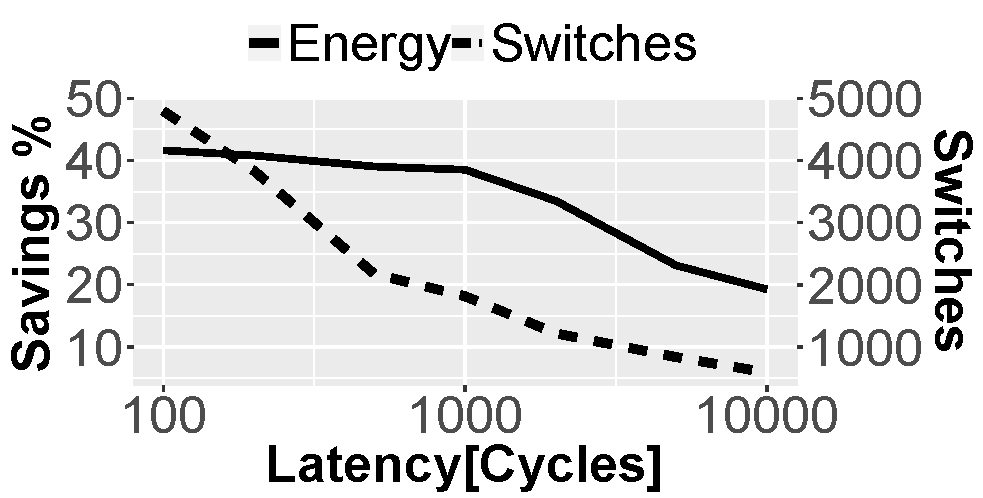
\includegraphics[width=.9\linewidth]{cases-paper/graphics/Exploration/latency_2.pdf}
    \caption{Energy savings and number of switches as a function of the switching latency in cycles.}
    \label{fig:enlatency}
\end{minipage}
\vspace{5mm}
\end{figure}

%Check if th
Up until now, the chapter has assumed a reconfiguration latency of 100 cycles whenever dynamic reconfiguration occurs, similar to~\cite{pricopi2012bahurupi} as explained in the background chapter, Chapter~\ref{chp:Background}.
This section studies the impact of a larger reconfiguration overhead on energy savings.
First, figure~\ref{fig:avlen} shows the average phase length for each benchmarks when maximising energy savings while maintaining performance (\textbf{DSpeed}).
As can be seen, the majority of the benchmarks run for long period of several ten of thousands cycles before any switching occurs.
Therefore, even if the reconfiguration latency is increased to a larger value (\eg 1,000 cycles), its impact might be minimal.
For these applications, the phase length is also tied to the size of the input, the phases may increase when working on inputs such as high definition images.

Furthermore, there is always the option to reconfigure less often, in the case where a change in configuration only brings marginal reduction in energy.
In such case it might be more beneficial to keep running on the slightly less optimal configuration than paying a cost for reconfiguration.
Figure~\ref{fig:enlatency} illustrates this perfectly, showing how energy behaves as a function of the reconfiguration overhead (averaged across benchmarks).
For each latency value, the best trace of reconfiguration is determined to keep performance constant while minimising energy (\textbf{DSpeed}).
The left y-axis expresses the energy savings relative to the static scheme, while the right y-axis shows the total number of switches.
The energy savings remains high up to a latency of 1,000 cycles, with a noticeable decrease in the number of switches.
For latency values over 1,000 cycles, the energy savings drop considerably, with very few switching occurring.
This data shows that even if the reconfiguration overhead is 1,000 cycles, average energy savings of 38\% are possible compared to 42\% when the overhead is 100 cycles.

\paragraph*{Summary}

Overall, dynamic core composition will always lead to higher speedup with lower energy consumption compared to a fixed configuration.
This is due to the presence of phases in applications that the dynamic scheme can exploit to reduce wasting energy in low ILP phases.
This section has shown that maximising speed can be highly energy inefficient when using a static composition and that a dynamic scheme can help reduce energy consumption by 42\% on average.

